\begin{topic}{Domain Name System}
\textbf{Distributed, hierarchical database} of \textbf{name servers} to map hostnames to IP addresses.

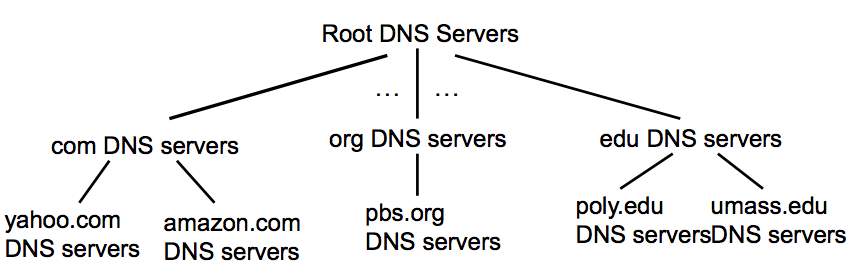
\includegraphics[scale=0.35]{coms3200/images/dnslayout}
\end{topic}

\begin{topic}{Name Servers}

\begin{subtopic}{1-}
\textbf{Root Name Servers}
13 root name servers worldwide map to TLD servers.
\end{subtopic}

\begin{subtopic}{2-}
\textbf{TLD Name Servers}
Responsible for mapping top-level domains such as com, org, edu, net to authoritative name servers.
\end{subtopic}

\begin{subtopic}{3-}
\textbf{Authoritative Name Servers}
An organizations name server, handles all domains below top-level.
\end{subtopic}

\begin{subtopic}{4-}
\textbf{Local Name Servers}
The default name server, stores local caches of DNS records for fast lookup. If a record cannot be founds, queries hierarchy.
\end{subtopic}

\end{topic}

\begin{topic}{DNS Resolution}
\begin{multicols}{2}
\textbf{Iterative Resolution}
Local server queries each server in the hierarchy for where to look next.
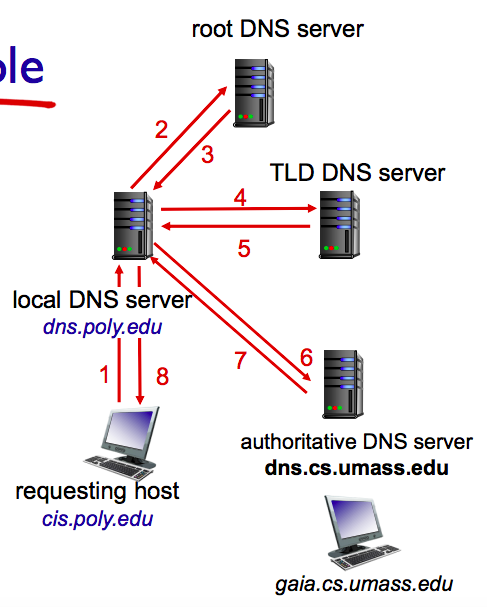
\includegraphics[scale=0.35]{coms3200/images/dnsresiter}

\columnbreak

\textbf{Recursive Resolution}
Hierachy name servers recursively query lower name servers.
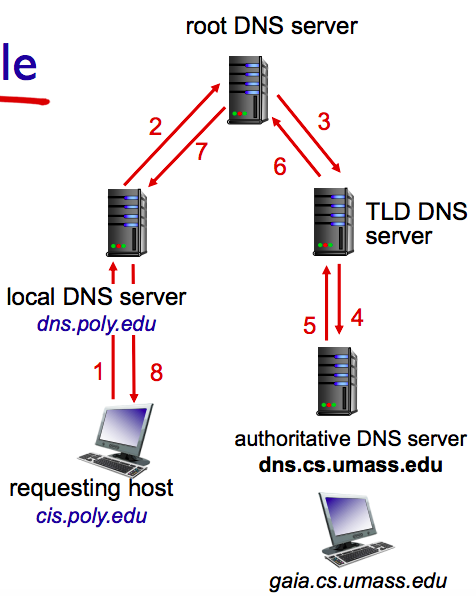
\includegraphics[scale=0.35]{coms3200/images/dnsresrec}
\end{multicols}

DNS records are cached by name servers for the particular records TTL.
\end{topic}

\begin{topic}{DNS Records}
DNS records are stored in a database as \textbf{resource records (RR)}

Format: (name, value, type, ttl)

\textbf{Type A:} name=hostname, value=ip address
\textbf{Type NS:} name=domain, value=authoritative name server for this domain
\textbf{Type CNAME:} name=alias hostname, value=real hostname
\textbf{Type MX:} name=hostname, value=mailserver
\end{topic}

\begin{topic}{DNS Attacks}
\begin{enumerate}
	\item bombard root name servers
	\item bombard tld name servers
	\item man-in-the-middle attacks: intercept queries
	\item DNS poisoning: send bogus information to DNS servers
	\item send queries with spoofed source address: target IP
\end{enumerate}
\end{topic}
